\documentclass[10pt, letterpaper]{article}
\usepackage[letterpaper,margin=0.75in]{geometry}
\usepackage{graphicx}
\usepackage{amsmath}
\usepackage{multirow}
\usepackage[table]{xcolor}
\setlength{\parindent}{0pt}
\setlength{\parskip}{5pt}
\renewcommand{\abstractname}{Overview}

\begin{document}

\title{CU Research Computing Allocation Request}
\author{Project Title Here}
\date{}
% Original draft, generated from pre-existing website content, by N. Featherstone, Jan 9, 2018
\maketitle


\begin{abstract}
\noindent Please fill out this template when constructing an allocation request for Summit.  Be sure to address all of the bullet points in this worksheet. If you feel that some of the requested information is not applicable, please note why that is rather than leaving that section out of your request entirely.
\\
\\
\noindent Requests for larger allocations will need more detailed justification. As a general guideline, a request for 300K SU might require a two-page proposal, while a 1M+ SU request might require three to five pages.
\\
\\
\noindent \textbf{If you have questions when preparing this allocation request, please contact rc-help@colorado.edu.  We are happy to provide advice and answer any questions.}

\end{abstract}
\section{Introduction and Summary}\label{sec:intro}
%\begin{center}
%\textit{(Suggested length: X pages)}
%\end{center}
Provide some background information on your proposal in this section.  Particularly:

\begin{itemize}
\item Concise Description - Describe the portion of the Project that this computational work supports.
\item Allocation goals - Describe the anticipated goals for this particular effort as a subset of the Project goals.
\item Duration: indicate if this allocation is for one year or until completion of a nearer-term goal whichever is sooner.
\item Expected follow-up - indicate if this is the final allocation for the Project or if work will likely continue.
\item Supporting grants - indicate funding agencies and grant numbers that support this work (if any).
\end{itemize}



%%%%%%%%%%%%%%%%%%%%%%%%%%%%%%%%%%%%%%%%%%%%%%%%%%%%%%%%%%%%%%%%%%%%%%%%%%%%%%%%%%%%%%%%%%%%%%%
%                                               Computational Details
\section{Computational Details}\label{sec:method}
%\begin{center}
%\textit{(Suggested length: X pages)}
%\end{center}

For cross-correlations of continuous seismic records, we use a parallel C++ application to calculate. The code was compiled using g++ compiler and -O3 flag. As for third-party libraries, it uses OpenMP runtime library. We run our code on shas partition, the cross-correlation code uses all the 24 cores on the each node. Our application doesn't require large amounts of RAM. Depending on the amount of data we assigned and nodes requested on each run, it typically take one day to one week for our jobs to run. Our application has well designed checkpoints, it can be restarted from a saved state. Our application is very I/O intense, the code checks the output files and continue the unfinished job from where it was terminated. We typically run our application on shas partition as our jobs don't require high memory and we are currently only using CPU to do the calculation. \\ \\
The other major application that we are going to run on Summit is a Monte-Carlo inversion code. The current version we plan to run is a parallel Python code. We are also going to run the inversion code on shas partition as it's not memory consuming. The inversion jobs usually run for several hours up to a week depending on the data size. \\ \\
The scaling information for these two applications we're going to use is provided below in Figure \ref{fig:scaling}. The applications we run are OpenMP parallel applications, so we only run our jobs on a single node. From the scaling results in Figure \ref{fig:scaling} which is a test run for single station inversion, we chose to use 24 cores for our jobs.

\begin{figure}
\centering
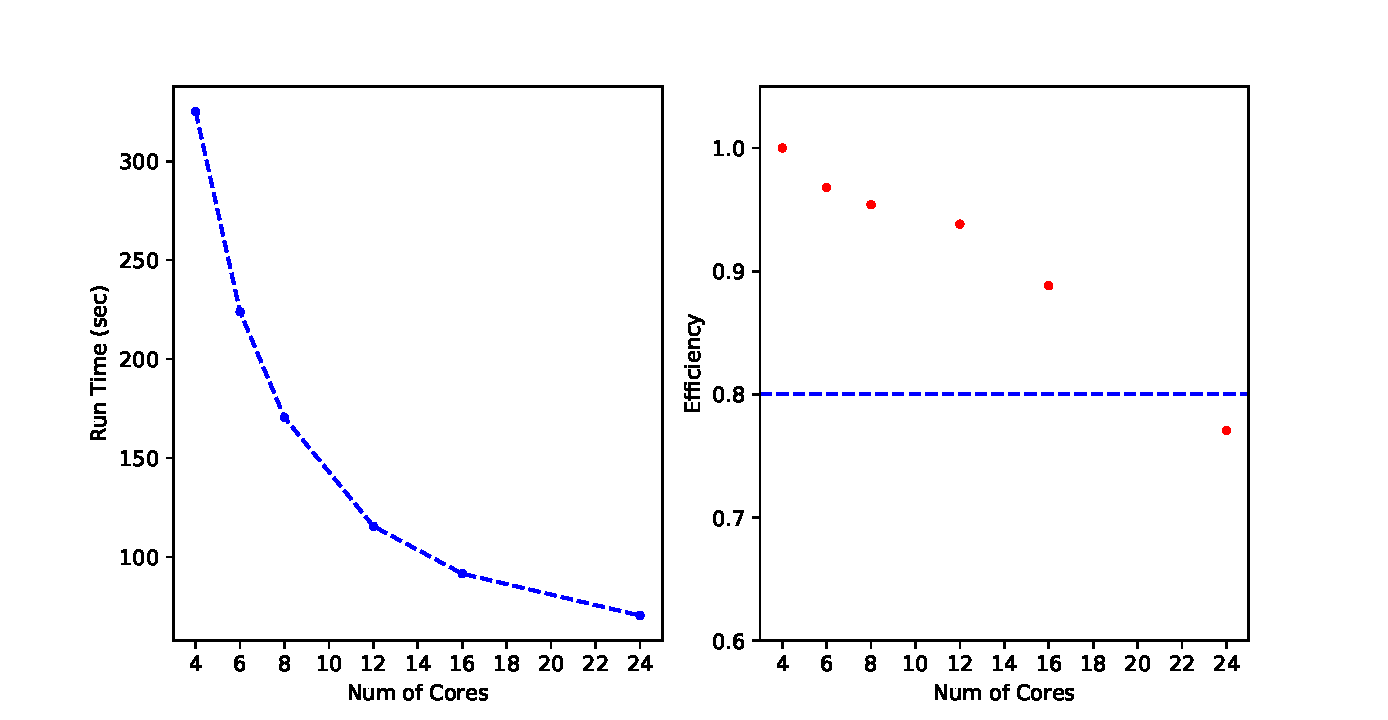
\includegraphics[width=\textwidth, keepaspectratio=true]{scaling.pdf}
\caption{\label{fig:scaling} Sample performance data for an example of test job run. (\textit{a}) Measured run time vs. number of cores.  (\textit{b}) Parallel efficiency as measured for different numbers of cores.}
\end{figure}

%%%%%%%%%%%%%%%%%%%%%%%%%%%%%%%%%%%%%%%%%%%%%%%%%%%%%%%%%%%%%%%%%%%%%%%%%%%%%%%%%%%%%%%%%%%%%%%
%                                               TIME REQUEST
\subsection{CPU Time Request}\label{sec:request}
%\begin{center}
%\textit{(Suggested length: X pages)}
%\end{center}

Our SU request detail is described in Table \ref{tab:worksheet}.

\begin{table}
\centering
\begin{tabular}{| c | c | c | c | c | c | c|}
\hline
 Job Type           & Node Type & Weight & Jobs  & Cores  & Hours & Total (SU)  \\\hline
Cross-Correlation   & shas      & 1      & 100    & 24     & 160   & 384,000 \\
Inversion           & shas      & 1      & 150   & 24     & 70    & 252,000 \\ 
Post-processing     & shas      & 1      & 200   & 24     & 2     & 9,600 \\\hline
Grand Total (SU)    & -         & -      &-      & -      &-      &  645,600 \\\hline
\end{tabular}
\caption{\label{tab:worksheet}SU request worksheet.}
\end{table}


%%%%%%%%%%%%%%%%%%%%%%%%%%%%%%%%%%%%%%%%%%%%%%%%%%%%%%%%%%%%%%%%%%%%%%%%%%%%%%%%%%%%%%%%%%%%%%%
%                                               I/O
\section{Data Management}\label{sec:IO}
%\begin{center}
%\textit{(Suggested length: X pages)}
%\end{center}
Our cross-correlation application is very I/O intensive. The typical job that we run each time has around 400 stations and each with 2 years of continuous data. We will have to request these continuous data from seismic data management centers, for data-set of such scale we expect 700 files each requires around 2GB space. From the original requested data, we extract daily 3-component seismic records this results in 1,400,000 files with size of around 2 MB each. We will then calculate cross-correlations between daily records from different stations, this will result in around 100,000,000 files and each file requires around 0.2 MB space. The original data that we requested will be removed after we calculate the daily cross-correlations (CC). We will stack the calculated daily cross-correlations to get our stacked CC products, for each job we expect to output 488,000 stacked files and each with around 0.2 MB size. All the I/O described here will be using /scratch storage. After we get the stacked CCs, we will make measurements on them and everything else on /scratch will be removed. \\ \\
The inversion application and other post-processing are not very I/O intensive, we incorporate Hierarchical Data Format (HDF) to store and organize the results. We use local disk for I/O and for each job we expect 2 or 3 files with size of several GB each. The stacked cross-correlations and inversion results will be migrated to our local computer and we will make backups on our local disks.

\begin{table}[h]
\centering
\begin{tabular}{| l | l | l |}
\hline
  Job Type            & Required Space (MB) & Number of Files  \\ \hline
  Requested  & 2,000                   &           700   \\
  Daily records  & 2                &             1,400,000   \\
  Daily CC & 0.2 & 116,800,000 \\
  Stacked CC & 0.2 & 488,000 \\
\hline
\end{tabular}
\caption{\label{tab:space}Scatch-disk-space requirements by job type.}
\end{table}

%%%%%%%%%%%%%%%%%%%%%%%%%%%%%%%%%%%%%%%%%%%%%%%%%%%%%%%%%%%%%%%%%%%%%%%%%%%%%%%%%%%%%%%%%%%%%%%
%                                               DATA MANAGEMENT
\end{document}
